\section{Methods} \label{RSS:sec:methods}

We first describe an approximation to the augmentation problem \eqref{RSS:eq:most_general}, which is specialized for manipulation. Next, we decompose this problem and describe each component in detail.

\subsection{Algorithm Overview}

Since robotic manipulation is interested specifically in moving objects, we focus on augmenting trajectories of poses and velocities of moving objects. A key insight is that objects in the scene can be categorized as either robots, moved objects, or stationary objects, and that these should be considered differently in augmentation. We denote the moved objects state as $\state$, the robot state as $\robot$, the robot action as $\action$, and the stationary objects as $\env$ (also called environment). Our method augments the moved object states, the robot state, and the actions, but not the stationary objects. We do not assume any specific representation for states or actions, and examples of possible representations include sets of points, joint angles, poses, or joint velocities. Since we operate on trajectories, we bold the state ($\bm{\state},\bm{\robot}$) and action ($\bm{\action}$) variables to indicate time-series (e.g $\state_{1:T}=\bm{\state}$). With this categorization, we can write $\example=\{\bm{\state},\bm{\robot},\bm{\action},\env\}$ and $\aug{\example}=\{\bm{\aug{\state}},\bm{\aug{\robot}},\bm{\aug{\action}},\env\}$.


We choose the parameters $\transform$ to be rigid body transformations, i.e. either $SE(2)$ or $SE(3)$. We parameterize $\transform$ as a vector with translation and rotation components, with the rotation component with Euler angles bounded from $-\pi/2$ to $\pi/2$, which gives uniqueness and a valid distance metric. These rigid body transforms are applied to moved objects in the scene, and augmented robot state and action are computed to match. We choose rigid body transforms because we can reasonably assume that even for articulated or deformable objects, augmenting with rigid body transforms preserve the internal forces, and therefore the augmentations are likely to be valid.

It may seem that an effective method to generate augmentations is then to randomly sample transforms independent of the data. However, this is not an effective strategy because it is highly unlikely to randomly sample valid and relevant transformations. We confirm this in our ablations studies (included in the Appendix 1.A). Instead of sampling transforms randomly, we formulate an approximation to Problem \ref{RSS:eq:most_general}:

\begin{equation}
    \label{RSS:eq:method}
    \begin{array}{cc}
        \underset{\transform}{\mathrm{min}} & 
        \lossDiversity(\transform,\target{\transform}) +
        \betaBbox\lossBbox(\bm{\aug{\state}}) + \betaValid\lossValid(\transform) + \\
        & \betaOcc\lossOcc(\bm{\aug{\state}},e) + \betaDmd\lossDmd(\bm{\aug{\state}},\env) + \\
        & \lossRobot(\bm{\aug{\state}},\bm{\aug{\robot}},\bm{\aug{\action}},\env) \\[1em]
        \text{subject to} & \{\bm{\aug{\state}},\bm{\aug{\robot}},\bm{\aug{\action}},\env\} = \apply(\bm{\state},\bm{\robot},\bm{\action},\env,\transform) \\
        & \target{\transform}\sim\transformUniform \\
    \end{array}
\end{equation}

The decision variable is now the parameters $\transform$, and the validity constraint is moved into the objective. We propose that diversity should be maximized by the transforms being uniformly distributed, and therefore $\lossDiversity$ penalizes the distance to a target transform $\target{\transform}$ sampled uniformly within $[\transform^-,\transform^+]$. The relevance and validity terms (which are intractable to compute) are replaced with four objective functions, which are specialized to manipulation. The magnitudes of different terms are balanced by ${\betaBbox,\betaValid,\betaOcc,\betaDmd}$, which are defined manually. We define each objective function below:

\subsubsection{Bounding Box Objective}
First is the bounding-box objective $\lossBbox$, which keeps the augmented states $\bm{\aug{\state}}$ within the workspace/scene bounds defined by $[\state^-,\state^+]$. The bounding box objective encourages relevance, since states outside the workspace are unlikely to be relevant for the task.

\begin{equation}
\lossBbox = \sum_{i=1}^{|s|}{\max(0,\bm{\aug{\state}}_i - \state^+_i) + \max(0,\state^-_i-\bm{\aug{\state}}_i)}
\end{equation}

\subsubsection{Transformation Validity Objective}
The transformation validity objective $\lossValid$ assigns high cost to transformations that are always invalid or irrelevant for the particular task or domain. It is defined by function $\validF$, which takes in only the transformation. For example, in our rope manipulation case, it is nearly always invalid to rotate the rope so that it floats sideways. In our cluttered pushing task, in contrast, this term has no effect. This term can be chosen manually on a per-task basis, but we also describe how a transformation validity objective can be learned from data in section \ref{RSS:sec:learnValid}.

\begin{equation}
\lossValid = \validF(\transform)
\end{equation}

\subsubsection{Occupancy Objective}
The occupancy objective $\lossOcc$ is designed to ensure validity by preventing objects that were separate in the original example from penetrating each other and ensuring that any existing penetrations are preserved. In other words, we ensure that the occupancy $O(p)$ of each point $\augStatePoint\in\augStatePoints$ in the augmented object state matches the occupancy of the corresponding original point $\statePoint\in\statePoints$. For this term, we directly define the gradient, which moves $\augStatePoint$ in the correct direction when the occupancies do not match. This involves converting the environment $\env$ into a signed-distance field (SDF) and the moved objects states $\bm{\state}$ into points $\statePoints$. This objective assumes that the environment has uniform friction, so that a contact/penetration in one region of the environment can be moved to another region.

\begin{equation}
\lossOcc=\sum_{\substack{\statePoint\in\statePoints \\ \augStatePoint\in\augStatePoints}} \SDF(\augStatePoint)\big(O(\statePoint)-O(\augStatePoint)\big)
\end{equation}

\subsubsection{Delta Minimum Distance Objective}
The delta minimum distance objective is designed to increase relevance by preserving near-contact events in the data. We preserve near-contact events because they may signify important parts of the task, such as being near a goal object or avoiding an obstacle. We define the point among the moved object points $\statePoints$ which has the minimum distance to the environment $\pointMinDist=\mathrm{argmin}_{\statePoint}\SDF(\statePoint)$. The corresponding point in the augmented example we call $\augPointMinDist$.

\begin{equation}
\lossDmd = ||\SDF(\pointMinDist)-\SDF(\augPointMinDist)||^2_2
\end{equation}


\begin{figure}
    \centering
    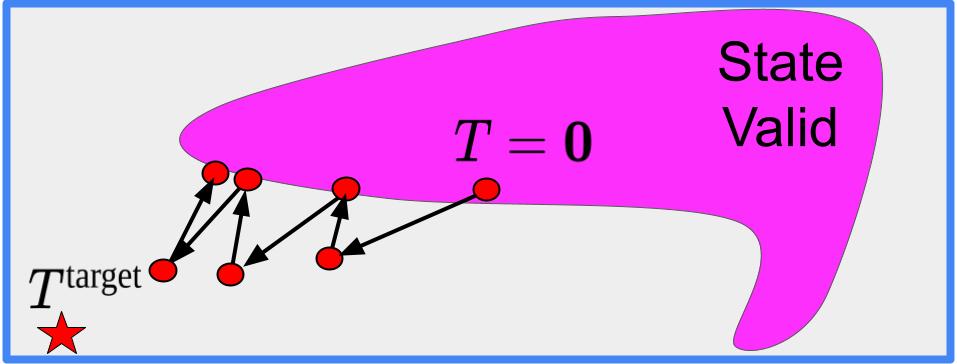
\includegraphics[width=0.5\linewidth]{Chap3/images/step_project.png}
    \caption{Illustration of \augState{} within Algorithm \ref{RSS:alg:aug}. All points and sets are in the space of $\transform$. The path of $\transform$ is shown in red with black arrows. The pink set, State Valid, is the set where \textit{state\_valid} is true. $\transform$ begins at the origin, and alternates between moving towards $\target{\transform}$ and projecting back into the set \textit{state\_valid} (by solving Equation \eqref{RSS:eq:project}).}
    \label{RSS:fig:step_project}
\end{figure}

\subsubsection{Robot Contact Objective}

The robot contact objective $\lossRobot$ ensures validity of the robot's state and the action. This means that contacts involving the moved objects which existed in the original example must also exist in the augmented example. Let the contact points on the robot be $\contactpoint_{\robot}$ and the contact points on the moved objects' state be $\contactpoint_{\state}$.

\begin{equation}
\lossRobot=\sum_i(||{\contactpoint_{\robot,i} - \contactpoint_{\state,i}}||^2_2)
\end{equation}

Finally, we note that other objective functions can be added for the purpose of preserving task-specific labels, i.e. so that $\ell(\example)=\ell(\aug{\example})$. However, for our experiments, no additional functions were necessary.

\subsection{Solving the Augmentation Optimization Problem}

This section describes how we solve Problem \eqref{RSS:eq:method}, and the procedure is detailed in Algorithm \ref{RSS:alg:aug}. First, we split the problem into two parts, \augState{} and \augRobot{}.

\begin{algorithm}[t]
\caption{$\augf(\bm{\state},\bm{\robot},\bm{\action},\env)$}\label{RSS:alg:aug}
\SetKwComment{Comment}{// }{}
\Comment{\augState{}}
$ \target{\transform} \sim \transformUniform $\\
$\transform = \mathbf{0}$ \text{ (identity)} \\
\For{$i \in \nStep$}{
    $\transform_\text{old}=\transform$ \\
    $\transform = \texttt{step\_towards}(\transform, \target{\transform})$ \\
    $\transform = $ solve Equation \eqref{RSS:eq:project} \\
    \If{$\distf{\transform} {\transform_\text{old}}<\projectionNotProgressing$}{
        break\\
    }
}
\Comment{\augRobot{}}
$\bm{\aug{\state}}, \textit{state\_valid} = \applyState(\bm{\state},\bm{\action},\transform)$\\
$\bm{\aug{\robot}},\bm{\aug{\action}}$, \textit{ik\_valid} $\leftarrow \mathrm{IK}(\bm{\robot},\bm{a},\bm{\aug{\state}},\env)$\\
\uIf{$!$state\_valid or $!$ik\_valid}{
    return $\bm{\state},\bm{\robot,}\bm{\action},\env$\\
}
\Else {
    return $\bm{\aug{\state}},\bm{\aug{\robot}},\bm{\aug{\action}},\env$\\
}
\end{algorithm}

In \augState{}, we optimize the transform $\transform$ to produce the moved objects' state $\bm{\aug{\state}}$ while considering environment $\env$. To achieve diversity, we uniformly sample a target transform $\target{\transform}$ and step towards it iteratively. This stepping alternates with optimizing for validity and relevance. We visualize this procedure in Figure \ref{RSS:fig:step_project}, as well as in the supplementary video. The innermost optimization problem is 
\begin{equation}
    \label{RSS:eq:project}
    \begin{array}{cc}
        \underset{\transform}{\mathrm{argmax}} & \betaBbox\lossBbox+\betaValid\lossValid+\betaOcc\lossOcc+\betaDmd\lossDmd \\
    \end{array}
\end{equation}

We solve Problem \eqref{RSS:eq:project} using gradient descent, terminating after either $\mProj$ steps or until the gradient is smaller than some threshold $\projStepSizeThreshold$.

Note that we start \augState{} in Algorithm \ref{RSS:alg:aug} with $\transform$ at the identity transformation, rather than initially sampling uniformly. This has two benefits. First, the identity transform gives the original example, which is always in the relevant set. Second, it is unlikely that a uniformly sampled transformation is valid or relevant, so starting at a random transformation would make solving Problem \eqref{RSS:eq:project} more difficult.

In \augRobot{}, we are optimizing $\lossRobot$. This corresponds to computing the augmented robot states $\bm{\aug{\robot}}$ and actions $\bm{\aug{\action}}$ given the augmented states $\bm{\aug{\state}}$ and the environment $\env$. Minimizing $\lossRobot$ means preserving the contacts the robot makes with the scene, which we do with inverse kinematics (Line 10 in Algorithm \ref{RSS:alg:aug}).

\subsection{Learning the Valid Transforms Objective}
\label{RSS:sec:learnValid}

As discussed above, we include a term $\lossValid$ based only on the transformation $\transform$. In some cases, such as our rope manipulation example, it may not be obvious how to define this objective manually. Our rope is very flexible, and therefore rotating the rope so that it floats in a sideways arc is invalid, but it may be valid for a stiff rope or cable. To address this, we offer a simple and data efficient algorithm for learning the transformation validity function $\validF$.

Our method for learning $\validF$ is given in Algorithm \ref{RSS:alg:valid_transformations_data}. This algorithm repeatedly samples augmentations of increasing magnitude, and tests them on the system (lines 6 and 8). This generates ground truth states starting from an input state and action. The result is a dataset $\learnValidDataset$ of examples ($\transform$, $\learnValidError$). We then train a small neural network $\learnedValidF$ to predict the error $\learnValidError$ and use the trained model as our transformation validity objective. We collect $\nLearnValid = \sqrt{10^\transformDim}$ examples, where $\transformDim$ is the dimensionality of the space of the transformation $\transform$.

\begin{algorithm}[t]
\caption{Data Collection for Learning Valid Transformations}\label{RSS:alg:valid_transformations_data}
\SetKwComment{Comment}{/* }{ */}
\KwIn{$\learnValidStateActionSet,\nLearnValid$}
\KwOut{$\learnValidDataset$}
$\minLearnValidError = \infty$ \\
\For{$i \in [1, \nLearnValid]$}{
    \For{$(\state_t,\robot_t,\action_t,\env) \in \learnValidStateActionSet$}{
        $ \learnValidScaling = i / \nLearnValid $ \\
        $ \transform \sim \mathbb{U}[\learnValidScaling\transform^-,\learnValidScaling\transform^+] $\\
        $ \state_{t+1}, \robot_{t+1} = \learnValidSimF(\state_t, \robot_t, \action_t, \env)$ \\
        $ \aug{\state}_{t,t+1}, \aug{\robot}_{t,t+1}, \aug{\action}_{t} = \apply(\state_{t,t+1},\robot_{t,t+1},\action_{t},\transform)$ \\
        $ \test{\aug{\state}_{t+1}}, \test{\aug{\robot}_{t+1}} = \learnValidSimF(\aug{\state_t}, \aug{\robot_t}, \aug{\action}_t, \env)$ \\
        $\learnValidError = || \aug{\state}_{t+1} - \test{\aug{\state}_{t+1}} ||$ \\
        \If {$\learnValidError < \minLearnValidError$}{
            $\minLearnValidError = \learnValidError,\,\transform_\text{min} = T,\,\minLearnValidError = \learnValidError$ \\
        }
    }
    add $(\transform_\text{min}, \minLearnValidError)$ to $\learnValidDataset$ \\
}
return $\learnValidDataset$
\end{algorithm}

This method owes its efficiency and simplicity to a few key assumptions about the system/data. First, we assume that we can collect a few ($<1000$) examples from the system and test various transformations. This could be performed in a simulator, as we do in our experiments. Because the transformation validity objective is not a function of state, action, or environment, we can make simplifications to this simulation by picking states and environments which are easy to simulate. We denote this set of states and actions as $\learnValidStateActionSet$. Second, because the transformation parameters are low-dimensional (3 and 6 in our experiments) the trained model generalizes well with relatively few examples.

\subsection{Application to Cluttered Planar Pushing}

In this section, we describe how we apply the proposed method to learning the dynamics of pushing of 9 cylinders on a table (Figure \ref{RSS:fig:sim_envs}). The moved object state $\state$ consists of the 2D positions and velocities of the cylinders. The robot state $\robot$ is a list of joint positions, and the actions $\action$ are desired end effector positions in 2D. There is no $\classLabel$ in this problem. The parameters $\transform$ used are $SE(2)$ transforms. In this problem, any individual trajectory may include some moved cylinders and some stationary ones. In our formulation, the stationary cylinders are part of $\env$ and are not augmented, whereas the moved ones are part of $\state$ and are augmented. The robot's end effector (also a cylinder) is also augmented, and IK can be used to solve for joint configurations which match the augmented cylinders' state and preserve the contacts between the robot and the moved cylinders.

\subsection{Application to Bimanual Rope Manipulation}

In this section, we describe how we apply the proposed method to a bimanual rope manipulation problem (Figure \ref{RSS:fig:sim_envs}). In this problem, there is a binary class label, so $\classLabel\in\{0,1\}$, which is preserved under our augmentation (last constraint in Problem \eqref{RSS:eq:most_general}). The rope is the moved object, and its state $\state$ is a set of 25 points in 3D. The robot state $\robot$ is a list of the 18 joint positions, and the actions $\action$ are desired end effector positions in the robot frame. In this problem, we know that the only contacts the robot makes with the objects or environment are its grasps on the rope. Therefore, we preserve these contacts by solving for a robot state and action that match the augmented points on the rope. The parameters $\transform$ used are $SE(3)$ transforms.

\begin{figure*}
    \centering
    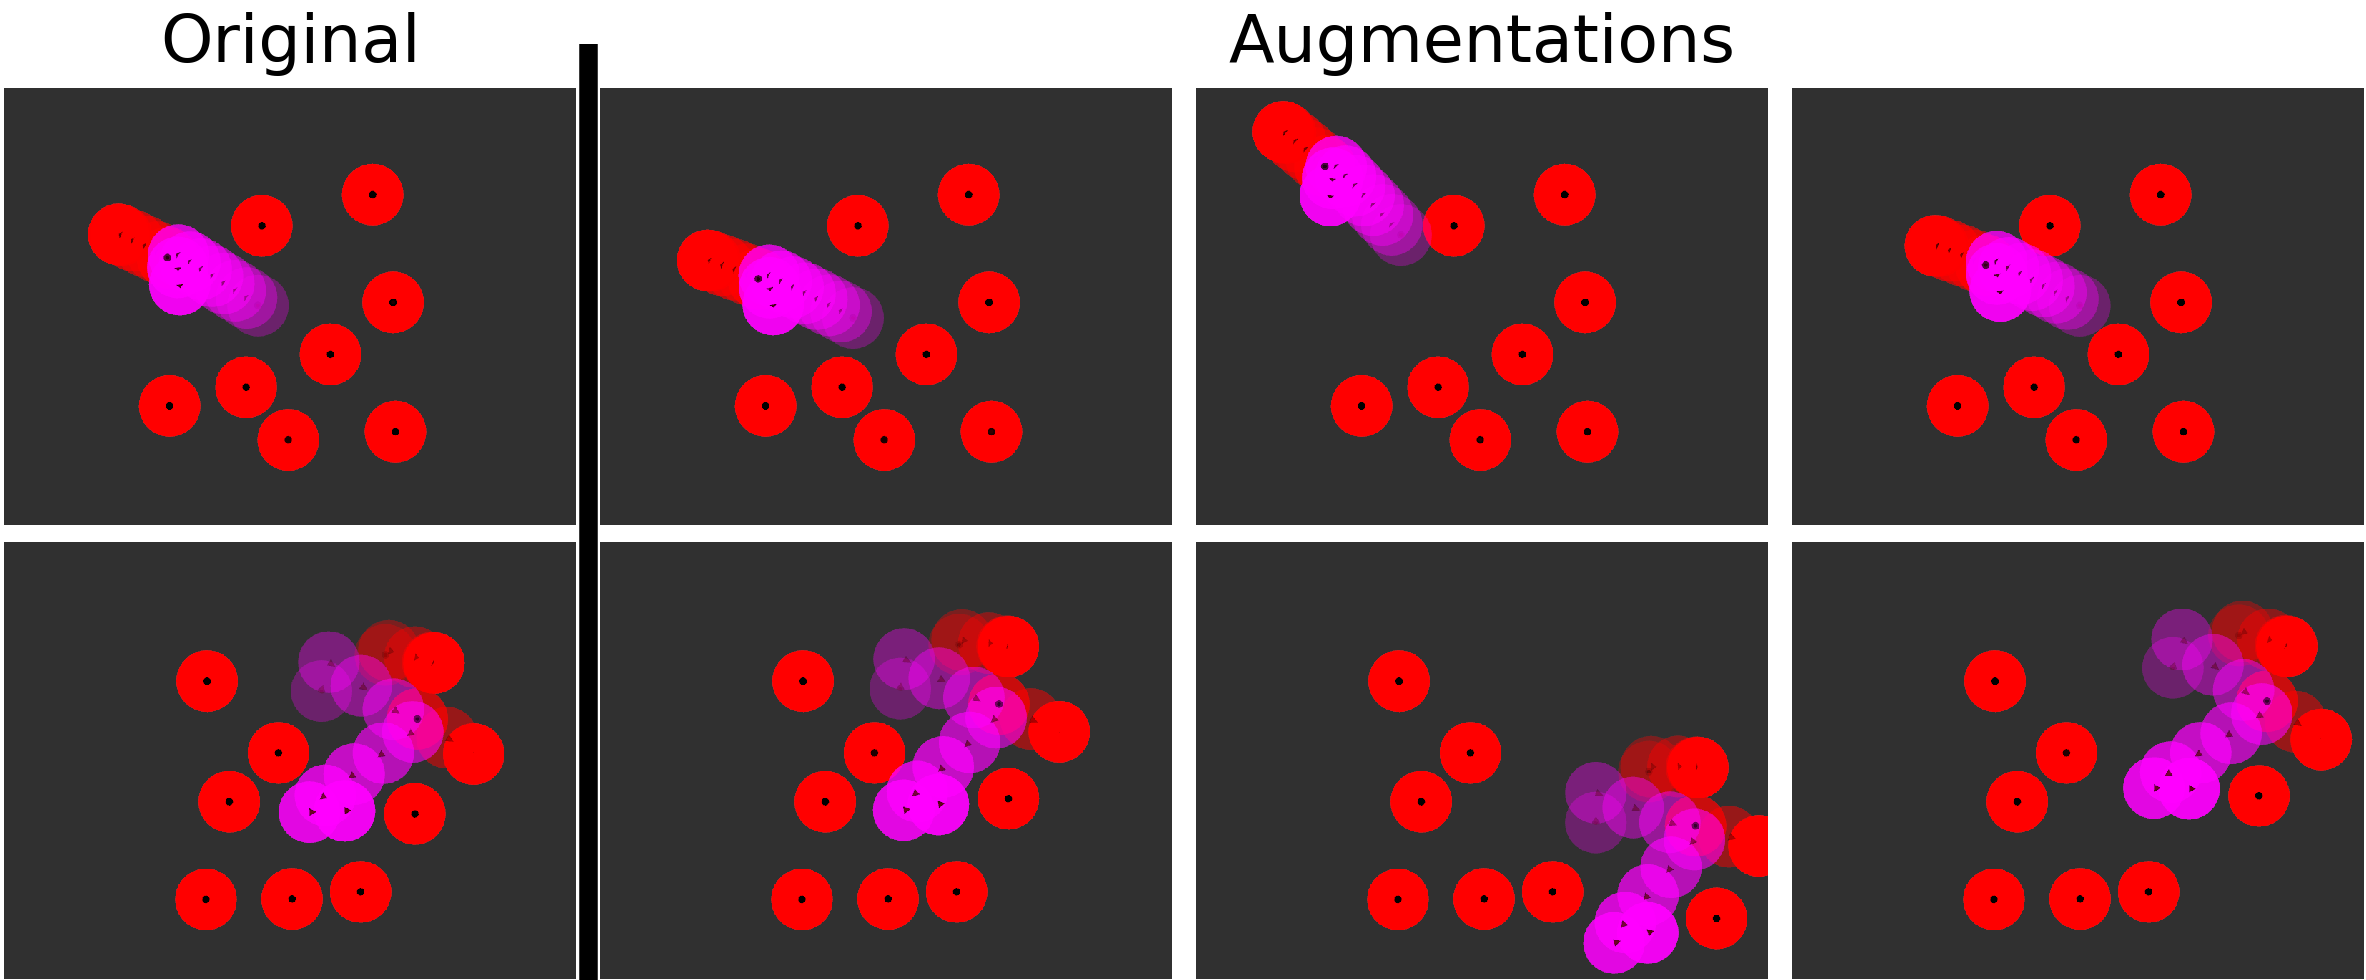
\includegraphics[width=1\linewidth]{Chap3/images/cylinders_aug_examples.png}
    \caption{Examples of augmentations generated for learning the dynamics of planar pushing of 9 cylinders. The pink cylinder is the robot. Time is indicated by transparency. Augmentation transforms the positions and velocities of the cylinders that moved, including the robot. All moved objects are transformed together, rigidly. Despite the clutter, we are able to find relatively large transformations that still preserve existing contacts but do not create any new ones.}
    \label{RSS:fig:cylinders_aug_examples}
\end{figure*}